%
% quantenfeldtheorie.tex -- Quantenfeldtheorie: Quantisierung, Schrödinger-Gleichung, der harmonische Oszillator, Photonen als Oszillatoren
%
% (c) 2020 Prof Dr Andreas Müller, Hochschule Rapperswil
%
% !TEX root = ../../buch.tex
% !TEX encoding = UTF-8
%
\section{Quantenfeldtheorie\label{fourier:section:quantenfeldtheorie}}
\kopfrechts{Quantenfeldtheorie}
Die beiden Wörter Quanten und Quantisierung ähneln sich, dessen Bedeutung jedenfalls nicht. 
Ein Quant ist ein kleinst mögliches Teilchen und Quantisierung bedeutet nichts anderes als zählbar. 
In der Quantenfeldtheorie ist genau dieser Schritt von zentraler Bedeutung, denn nun ist alles zählbar. 
Dabei werden klassische Felder wie das elektromagnetische Feld in quantenmechanische Operatoren überführt, wodurch die zuvor kontinuierlichen Felder plötzlich aus einer endlichen Menge von Quanten bestehen.

Wie kam es eigentlich dazu, dass man physikalische Größen plötzlich als „quantisiert“ betrachtete?
Ein kurzer Blick in die Geschichte hilft, diesen Schritt besser zu verstehen.

\subsection{Die Idee der Quantisierung\label{fourier:subsection:DieIdeeDerQuantisierung}}
	Mit 16 Jahren fragte Max Planck seinen Professor, ob sich ein Studium in der Physik lohne. 
	Dieser antwortete:
	
	\begin{center}
		\textit{``{}In diesem Fach ist im Grunde schon alles entdeckt, was es zu entdecken gibt.
		Es bleibt höchstens noch, ein paar Lücken auszufüllen. ''}
	\end{center}
	
	Das war 1874.
	Zum Glück liess sich Planck davon nicht abhalten.
	1897 wurde er Professor für Physik und beschäftigte sich mit einem dieser ungelösten Probleme, der Schwarzkörperstrahlung, auch bekannt als die Ultraviolette katastrophe. 
	
	
	In der Abbildung~\ref{fourier:fig:schwarzkoerper} ist das Experiment dargestellt. Ein hohler Metallwürfel mit einem Loch wird erwährmt. Die ganze Elektromagnetische Strahlung die von aussen in das Loch eindringt wird im inneren absorbiert, siehe blauer Pfeil. Die austretende Strahlung wird somit nur vom Würfel abgegeben, siehe die roten Pfeile. Der Schwarze Strahler ist in Wirklichkeit das Loch und nicht das Material selbst, obschon man dazu ein geeignetes Material benötigt! Nun misst man welche Intensität von welcher Wellenlänge aus dem Loch ausdringt, diese hängt auch von der Temperatur des Eisenblock ab. 
	Gut zu wissen ist, dass jedes Objekt über dem absoluten Nullpunkt elektromagnetische Wellen abstrahlt. 
	Sehen tut man dies normalerweise nicht, da sich zu wenig Strahlung im Sichtbaren Wellenbereich, zwischen 400nm und 780nm, befindet. 
	
	\input{papers/fourier/fig/fig-schwarzkoerper.tex}
	
	In der Abbildung~\ref{fourier:fig:strahlungsspektren} wurde der Eisenblock auf 1000K erwährmt und anschliessend gemessen wie hoch die Intensität bei jeder Wellenlänge ist. 
	Die Messwerte liegen auf der schwarzen Kurve.
	Bei dieser Temeratur ist glüht das Eisen Rötlich, hiermit handelt es sich um vom Bock abgegebene elektromagnetsiche strahlung!
	
	
	Nach dem Rayleigh-Jeans-Gesetz 
	
	\begin{equation}
		B(\lambda, T) = \frac{2 \pi c k_\mathrm{B} T}{\lambda^4}
	\end{equation}
	
	steigt die abgegebene Strahlung eines Körpers mit kleiner werdender Wellenlänge immer weiter an. 
	Bei hohen Wellenlängen passt das Gesetz gut, aber im ultravioletten Bereich versagt die Theorie komplett. Ultraviolette Strahlung umfasst den Wellenbereich von 10 nm bis 400 nm. 
	Dieses Spektrum befindet sich auf der linken Seite.
	Die Formel sagt gigantische Energien voraus, während in Wirklichkeit kaum noch Strahlung messbar ist.
	Planck suchte drei Jahre lang nach einer Lösung, einer neuen Erkenntnis, aus der er eine neue Formel aufstellen kann, die korrekt ist. 
	Leider funktioniert dies nicht.
	
	
	Am Ende war es eher ein Akt der Verzweiflung als eine geniale Eingebung. Er suchte nicht mehr nach einer neuen Theorie, sondern nach einem mathematischen Trick, der zu den Messwerten passte. 
	Dabei wusste er nicht, was seine Formel physikalisch bedeutete.
	So entstand diese Formel: 
	
	\begin{equation}
		B(\lambda, T) = \frac{2 \pi h c^2}{\lambda^5} \cdot \frac{1}{e^{\frac{h c}{\lambda k_B T}} - 1}
	\end{equation}
	
	Mithilfe der exponential Funktion geht nun die Intensität gegen Null, bei tiefen Wellenlängen. Ausserdem benötige er noch eine konstante $h$. Heutzutage ist $h$ eine Naturkonstante und bekannt als das Plancksche Wirkungsquantum $h = 6{,}626 \cdot 10^{-34} \ \text{J\,s}$. 
	

	%https://de.wikipedia.org/wiki/Rayleigh-Jeans-Gesetz#/media/Datei:PlanckWienRayleigh_linear_150dpi_de.png

	%
% fig-strahlungsspektren.tex
%
% (c) 2025 Prof Dr Andreas Müller
%
\begin{figure}
\centering
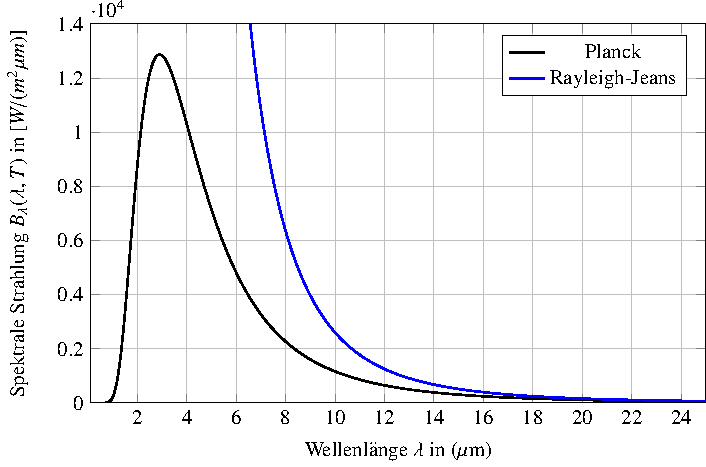
\includegraphics{papers/fourier/images/strahlung.pdf}
\caption{Vergleich der Strahlungsspektren nach Planck und nach Rayleigh–Jeans für einen auf 1000 K erhitzten Metallblock.%
\label{fourier:fig:strahlungsspektren}}
\end{figure}
	
	
	Früher nahm man an, die Energie einer Welle hänge nur von ihrer Amplitude ab. 
	Man glaubte auch, Atome könnten jede beliebige Energiemenge abstrahlen. 
	Plancks Modell stellte das infrage. 
	Nun konnte Energie nur in bestimmten Portionen abgegeben werden, abhängig von der Frequenz und nicht von der Amplitude. 
	Dieser Zusammenhang lässt sich mit
	
	\begin{equation}
		E = h \cdot f
	\end{equation}
	
	 ausdrücken, die frequenz mulitipliziert mit dem Planckschem Wirkungsquantum ergiebt die Energie.
	 Oft wird diesebe Formel mit dem reduzierte Plancksche Wirkungsquantum $\hbar = \frac{h}{2\pi}$ und der Winkelgeschwindigkeit $\omega = 2 \pi f$ ausgedrückt:
	 
	 \begin{equation}
		E = \frac{h}{2\pi} \cdot 2\pi f = \hbar \cdot \omega
	 \end{equation}
	 
	 
	Je höher die Frequenz, desto grösser ist das nötige Energiepaket. 
	Deshalb nimmt die Strahlung bei hohen Frequenzen wieder ab, denn hohe Frequenzen bedeuten viel Energie pro Lichtquant und es ist ziemlich unwahrscheinlich, dass ein einzelnes Atom so viel Energie auf einen Schlag abgibt. 
	Planck wusste dies nicht. 
	Aber mit dieser Formel war der erste Schritt in Richtung Quantentheorie gemacht.
	Ausserdem lässt sich nun die frage aus Kapitel~\ref{fourier:section:AnwendungAufFeld} beantworten. 
	Die Frage war ob unendlich Frequenzen möglich sind, da bei der Fourier-Reihe die Frequenzen bis ins Unendliche ansteigten. 
	Die Antwort ist einfach mit der obrigen Formel zu beantworten, wenn die Frequenz nach unendlich geht, so wird die Energie auch nach unendlich gehen, was nicht möglich ist.

	
	%Einstein
	
	
	1905 kam Albert Einstein ins Spiel. 
	Er griff diese Formel auf, um den photoelektrischen Effekt zu erklären. 
	Er interpretierte sie so, dass Elektromagnetische Strahlung tatsächlich aus Teilchen (Photonen) besteht, die jeweils die Energie $E = h \cdot f$ tragen, also nicht nur als mathematischer Trick wie bei Planck, sondern als reale physikalische Aussage über die Natur von Elektromagnetischer Strahlung.
	Für diese Arbeit bekam er 1921 den Nobelpreis und nicht für seine Relativitätstheorie, wie viele denken.
	
	 
	%Bohr
	
	%Auskommentier, da exkurs (Atommodell)
	
	%1913 übertrug Niels Bohr die Quantisierung auf Atome. 
	%In seinem Modell befinden sich Elektronen in Schalen, dazuwischen ist nichts. 
	%Ein Übergang zwischen diesen diskreten Schalen ging immer mit einer Energieabgabe oder aufnahme in Form eines Photons einher. 
	%Auch wenn sein Modell längst überholt ist, war seine Idee von Schalen Grundlegend korrekt. 

	%de Broglie
	
	1924 stellte Louis de Broglie eine revolutionäre Idee vor.
	Nicht nur elektromagnetische Strahlung besitzt Wellencharakten, auch Materie, also Teilchen wie Elektronen, könnten wellenartige Eigenschaften haben.
	Er vermutete, dass jedem Teilchen mit Impuls p eine Wellenlänge λ zugeordnet werden kann:
	
	\begin{equation}
		\lambda = \frac{h}{p}
	\end{equation}	
	
	Mit dieser einfachen Formel verband de Broglie die Vorstellung von Teilchen und Wellen. Damit wurde erstmals verständlich, warum sich auch Elektronen in bestimmten Experimenten wie Wellen verhalten.
	Kurios ist, dass jedes Objekt eine Wellenlänge hat, auch ein Fussball.
	Angenommen man schiesst ein Fussball mit der Masse von 0.45 \text{kg} mit der Geschwindigkeit von 20 \text{m/s}.
	
	\begin{equation}
		\lambda = \frac{h}{p} = \frac{h}{m \cdot v} = 	\frac{6{,}626 \cdot 10^{-34} \ \text{Js}}{0{,}45 \ \text{kg} \cdot 20 \ \text{m/s}} \approx 7{,}36 \cdot 10^{-35} \ \text{m}
	\end{equation}	
	
	Die Berechnung zeigt, dass der Fussball eine extrem kleine Wellenlänge hat, somit besitzt er Wellencharakteristiken.
	Das Resultat ist absurd und hat in der Realität keinerlei bedeutung.
	Solche Rechnungen machen nur in der Quantenwelt Sinn, auch wenn die Gleichungen für alle Objekte gelten. 
	De Broglie zeigte, dass Wellen als Teilchen intepretiert werden können und umgekehrt. 
	
	
	
	%Schrödinger
	Erwin Schrödinger formulierte 1926 eine Gleichung, die das Verhalten von Teilchen als Wellen beschreibt. 
	Sie bildet die Grundlage der Quantenmechanik. Die Lösung dieser Gleichung ist die Wellenfunktion \( \psi(x, t) \). Sie liefert keine feste Bahn, sondern eine Wahrscheinlichkeitsverteilung für den Aufenthaltsort eines Teilchens.
	Die eindimensionale zeitabhängige Schrödinger-Gleichung lautet:
	
	\begin{equation}\label{fourier:equation:zeitabhaengigeSchroedingerGleichung}
		i \hbar \frac{\partial \psi(x,t)}{\partial t} = -\frac{\hbar^2}{2m} \frac{\partial^2 \psi(x,t)}{\partial x^2} + V(x) \psi(x,t)
	\end{equation}
	
	
	Um herauszufinden, wie wahrscheinlich ein Teilchen an einem Ort ist, muss man den Betrag von $\psi(x, t)$ quadrieren. 
	Die resultierende Funktion $|\psi(x, t)|^2$ ist die Aufenthaltswahrscheinlichkeit. 
	
	Die Reise begann mit Plancks Energiepaketen, führte über Einsteins Lichtteilchen und de Broglies Materiewellen hin zu Schrödingers Wahrscheinlichkeitswellen. 
	Doch all diese Ideen behandelten Teilchen meist als isolierte Objekte.
	Die Quantenfeldtheorie geht einen Schritt weiter.
	Sie besagt, dass Teilchen nicht mehr als kleine Kügelchen existieren, sondern als Anregungen von Feldern, die den gesamten Raum durchdringen. 
	Elektronen, Photonen und alle anderen Teilchen sind Wellen in ihren jeweiligen Quantenfeldern.
	Damit verschmilzt die Teilchenwelt mit der Feldvorstellung.
	Nicht das Teilchen ist grundlegend, sondern das Feld und was wir beobachten, sind nur dessen kleinste Schwingungen.
	So wird aus der Quantenmechanik eine Feldtheorie.
	
	\subsection{Der quantenmechanische harmonische Oszillator\label{fourier:subsection:derQMHarmonischeOszillator}}

	Im Kapitel~\ref{fourier:section:AnwendungAufFeld} wurde gezeigt, wie sich eine klassische Wellengleichung mithilfe einer Fourierzerlegung in eine Überlagerung von Schwingungsmoden zerlegen lässt.
	Jede dieser Moden erfüllt formal die Bewegungsgleichung eines klassischen harmonischen Oszillators.

	Kapitel~\ref{fourier:section:derKlassischeHarmonischeOszillator} untersuchte diesen Fall genauer:
	Die Gesamtenergie eines solchen Oszillators setzt sich zusammen aus kinetischer Energie \( \frac{p^2}{2m} \) und potentieller Energie \( \frac{1}{2}kx^2 \).
	Damit ergibt sich die klassische Energieformel:
	\begin{equation}
	E = \frac{p^2}{2m} + \frac{1}{2}kx^2.
	\end{equation}

	Im vorherigen Abschnitt~\ref{fourier:section:quantenfeldtheorie} wurde schließlich beschrieben, wie in der Quantenfeldtheorie klassische Felder in quantenmechanische Operatoren überführt werden.
	Genau diesen Übergang wollen wir nun am Beispiel eines einzelnen harmonischen Oszillators nachvollziehen.

	\vspace{1em}

	In der Quantenmechanik wird die Energie nicht mehr durch eine Zahl beschrieben, sondern durch einen Operator.
	Die klassische Energieformel führt uns dabei direkt zum sogenannten \emph{Hamilton-Operator}:
	\begin{equation}
	\hat{H} = \frac{\hat{p}^2}{2m} + \frac{1}{2} k \hat{x}^2.
	\label{fourier:equation:derQMHO}
	\end{equation}

	Physikalisch messbare Größen wie Ort, Impuls oder Energie werden nun durch Operatoren beschrieben.
	Diese wirken auf einen sogenannten \emph{Hilbertraum} — den Raum aller quantenmechanischen Zustände.
	Die erlaubten Messwerte sind die Eigenwerte dieser Operatoren.
	Im Fall des harmonischen Oszillators ergibt sich ein \emph{diskretes Energiespektrum}:
	\[
	E_n = \hbar \omega \left(n + \frac{1}{2} \right), \quad n = 0, 1, 2, \dots
	\]

	Die Energie des Systems ist damit nicht mehr beliebig, sondern in diskrete Stufen unterteilt.
	Der Oszillator kann nur auf bestimmten, gleichmäßig verteilten Niveaus existieren.
	Warum hier ein zusätzlicher Term $\frac{1}{2}$ auftritt, wird im Kapitel~\ref{fourier:subsection:Leiteroperatoren} genauer erklärt.

	Der harmonische Oszillator spielt in der Quantenphysik eine fundamentale Rolle.
	Das liegt nicht nur an seiner mathematischen Einfachheit, sondern auch daran, dass viele physikalische Systeme — zumindest näherungsweise — durch ihn beschrieben werden können.

	Die Quantisierung des harmonischen Oszillators ist damit nicht nur ein mathematisches Spiel, sondern der Grundbaustein für das Verständnis der modernen Quantenfeldtheorie.
	Ein besonders wichtiges Beispiel ist das elektromagnetische Feld:
	Wie bereits in Kapitel~\ref{fourier:section:AnwendungAufFeld} gesehen, lässt sich dieses Feld als Summe von Moden darstellen.
	Jede dieser Moden entspricht einem quantenmechanischen Oszillator.
	Die Zustände dieser Oszillatoren — sogenannte Photonenzahlenzustände — erklären, warum Licht nicht kontinuierlich, sondern in diskreten Paketen (Photonen) emittiert und absorbiert wird.
	Darüber hinaus findet der quantenmechanische harmonische Oszillator auch in vielen anderen Bereichen Anwendung:
	In der Festkörperphysik beschreibt er beispielsweise die Gitterschwingungen (Phononen), während er in der Quantenoptik zur Modellierung von Lichtfeldern dient.
	Sogar in der Elektrotechnik ist das Konzept grundlegend ---
	etwa bei der Beschreibung von Resonanzphänomenen in elektrischen Schaltkreisen oder der Analyse schwingungsfähiger Systeme.

\subsection{Einführung in Werkzeuge der Quantenmechanik\label{fourier:subsection:werkzeugeQuantenmechanik}}
	Die bisherige Entwicklung --- von Plancks Energiepaketen über Einsteins Lichtquanten bis hin zu Schrödingers Wellenfunktion ---
	macht deutlich, dass die Beschreibung von Ort, Impuls und Energie in der Quantenmechanik völlig neue mathematische Werkzeuge und Denkweisen erfordert.
	An die Stelle klassischer Teilchenbahnen treten in der Quantenmechanik Wahrscheinlichkeiten, Operatoren und Zustandsräume.

	In den folgenden Abschnitten werden drei grundlegende Konzepte vorgestellt:
	\begin{itemize}
	\item \textbf{Bra-Ket-Notation}:
	Dient zur kompakten Darstellung von Zuständen und Operatoren im Hilbertraum.

	\item \textbf{Heisenbergsche Unschärferelation}:
	Beschreibt die fundamentale Grenze der gleichzeitigen Bestimmbarkeit von Ort und Impuls.

	\item \textbf{Hamilton-Operator und Schrödinger-Gleichung}:
	Zwei zentrale mathematische Werkzeuge, mit denen sich die Dynamik quantenmechanischer Systeme vollständig beschreiben lässt.
	\end{itemize}

	Diese Konzepte sind nicht nur theoretisch relevant, sondern bilden die Grundlage für das Verständnis von Photonen, Feldern und quantisierten Schwingungen im weiteren Verlauf.

	\subsubsection{Bra-Ket-Notation\label{fourier:subsubsection:braKetNotation}}
		Die Bra-Ket-Notation, auch Dirac-Notation genannt, wurde von Paul Dirac eingeführt und ist heute Standard in der Quantenmechanik.
		Sie dient dazu, Zustände und Operatoren kompakt und elegant darzustellen.

		Ein \emph{Ket} $|\psi\rangle$ beschreibt den Zustand eines quantenmechanischen Systems.
		Man kann sich Kets wie Richtungspfeile oder Vektoren vorstellen, die angeben, in welchem Zustand sich das System gerade befindet ---
		zum Beispiel mit welchem Energieeigenwert, welcher Spinquantenzahl oder an welchem Ort sich ein Teilchen befindet.	Ein \emph{Bra} $\langle\psi|$ ist das zugehörige Dualelement zum Ket.
		Es steht symbolisch für eine Messung oder einen Test auf diesen Zustand.
		Formal ist es das komplex-konjugierte und transponierte Objekt zum Ket.

		Beispiele:
		\begin{itemize}
		\item $|0\rangle$ kann den Grundzustand eines Systems beschreiben.
		\item $|x\rangle$ steht für einen Zustand, in dem sich ein Teilchen genau am Ort $x$ befindet.
		\item Allgemeine Zustände lassen sich als Superposition (Überlagerung) schreiben, z.B.:
		\[
			|\psi\rangle = \alpha\,|0\rangle + \beta\,|1\rangle,
		\]
		wobei $\alpha$ und $\beta$ komplexe Zahlen sind.
		\end{itemize}

		Das \emph{Skalarprodukt}
		\begin{equation}
		\langle \varphi | \psi \rangle = \int\limits_{-\infty}^{+\infty} \varphi^*(x)\,\psi(x)\,dx,
		\end{equation}
		ist eine einzige (meist komplexe) Zahl, die angibt, wie ``gleich'' oder ``verschieden'' sich die beiden Zustände $|\varphi\rangle$ und $|\psi\rangle$ verhalten.
		Man multipliziert dafür $\varphi^*(x)$ (das konjugiert-komplexe von $\varphi$) mit $\psi(x)$ und integriert über den gesamten Raum.
		\begin{itemize}
			\item Liegen die Zustände ``genau übereinander'', erhält man den Betrag 1 (bei Normierung).
			\item Sind sie orthogonal, also völlig verschieden, ist das Ergebnis 0.
		\end{itemize}
		Kurz gesagt:
		$\langle \varphi | \psi \rangle$ misst die Überlappung (den ``Winkel'') zwischen zwei Quantenzuständen.

		Die \emph{Norm} eines Zustands ist einfach das Skalarprodukt mit sich selbst:
		\begin{equation}
		\langle \psi | \psi \rangle = \int \psi^*(x)\,\psi(x)\,dx.
		\end{equation}

		Der \emph{Erwartungswert} eines physikalischen Operators $A$ im Zustand $|\psi\rangle$ beschreibt den durchschnittlich gemessenen Wert bei vielen Wiederholungen:
		\begin{equation}
		\langle A \rangle = \langle \psi | A | \psi \rangle = \int \psi^*(x)\,(A\psi)(x)\,dx.
		\end{equation}
		Dabei wirkt der Operator $A$ auf den rechten Ket und das Ergebnis wird mit dem Bra skalar multipliziert.
		
		Ist $|\psi\rangle$ ein Eigenzustand von $A$ mit einem bestimmten Eigenwert $a$, d.h.
		\begin{equation}
		A\,|\psi\rangle = a\,|\psi\rangle,
		\end{equation}
		so ergibt eine ideale Messung des Operators $A$ immer genau den Wert $a$.

		Die Bra-Ket-Notation ist nicht nur kompakt, sondern macht viele Rechnungen in der Quantenmechanik übersichtlich und leicht handhabbar.

	\subsubsection{Heisenbergs Unschärferelation%
	\label{fourier:subsubsection:unschaerferelation}}
	In der Quantenmechanik gibt es keine festen Werte für Grössen wie Ort oder Impuls eines Teilchens, sondern nur Wahrscheinlichkeiten und Mittelwerte, wo sich diese befinden oder wie schnell sie sind.
	Im Gegensatz zur klassischen Physik, wo der Impuls $p$ eine klar definierte Zahl ist, wird in der Quantenmechanik der Impuls durch einen sogenannten Operator beschrieben:
	\begin{equation}
		\hat{p} = \frac{\hbar}{i} \frac{d}{dx}.
	\end{equation}
	Das bedeutet:
	Man kann nicht einfach sagen ``Das Teilchen hat genau diesen Impuls'', sondern der Impuls ist grundsätzlich unscharf (nicht exakt bestimmbar).
	Ort und Impuls sind sogenannte nicht gleichzeitig messbare Grössen:
	Ihre Operatoren ``vertauschen'' nicht miteinander, was mathematisch ausgedrückt wird durch
	\begin{equation}
		[\hat{x},\hat{p}] = \hat{x} \hat{p} - \hat{p} \hat{x} = i \hbar.
	\end{equation}
	Diese fehlende Vertauschbarkeit führt direkt zur bekannten Unschärferelation.
	Ihre Herleitung basiert auf einer grundlegenden mathematischen Ungleichung, der sogenannten Cauchy-Schwarz-Ungleichung:
	\begin{equation}
		\vec{a} \bullet \vec{b} = |\vec{a}| |\vec{b}|\cos\alpha \le |\vec{a}| |\vec{b}|.
	\end{equation}
	die besagt, dass das Skalarprodukt zweier Vektoren nie grösser sein kann als das Produkt ihrer Längen.
	Übertragen auf die Wellenfunktionen zweier Quantenzustände $|\varphi\rangle$ und $|\chi\rangle$, erhält man
	\begin{equation}
		|\langle\varphi | \chi\rangle|^2 \le \langle\varphi | \varphi\rangle \langle\chi | \chi\rangle.
	\end{equation}
	Diese Relation setzt eine obere Schranke dafür, wie stark zwei Zustände miteinander überlappen können. Sie beschreibt also, wie ähnlich sich zwei Zustände in ihrer quantenmechanischen Beschreibung überhaupt sein können.
	Der Ausdruck $|\langle\varphi|\chi\rangle|^2$ misst die Überlappung der beiden Zustände, also gewissermaßen, wie ähnlich sie sich sind.
	Die Terme $\langle\varphi|\varphi\rangle$ und $\langle\chi|\chi\rangle$ entsprechen dabei den Quadraten der Längen (Normen) der Zustände.
	Der Betrag des Skalarprodukts kann also niemals größer werden als das Produkt der Normen, ganz analog zur klassischen Vektoranalysis.
	Das Quadrat auf der linken Seite ergibt sich, weil die Ungleichung eine Aussage über den Betrag des Skalarprodukts ist, während die rechte Seite stets reell und positiv ist.
	Diese Form der Ungleichung bildet die mathematische Grundlage für die Herleitung der heisenbergschen Unschärferelation.
	Die Zustände $|\varphi\rangle$ und $|\chi\rangle$ sind hier in der Bra-Ket-Notation geschrieben, einer kompakten Notation für Zustände in der Quantenmechanik, wie sie in Abschnitt~\ref{fourier:subsubsection:braKetNotation} eingeführt wurde.

	Setzt man
	\begin{equation}
		|\varphi\rangle = (\hat{x} - \langle \hat{x} \rangle) |\psi\rangle \quad |\chi\rangle = (\hat{p} - \langle \hat{p} \rangle) | \psi\rangle,
	\end{equation}
	also die Abweichungen von Ort und Impuls gegenüber ihren Mittelwerten ein, so führen die Definitionen
	\begin{equation}
		\sigma_x^2 = \langle\varphi | \varphi\rangle \text{ und } \sigma_p^2 = \langle\chi | \chi\rangle
	\end{equation}
	für die sogenannten Standardabweichungen --- ein Mass für die „Streuung“ oder Unschärfe --- zusammen mit
	\begin{equation}
		\langle\psi | [\hat{x},\hat{p}] | \psi\rangle = i\hbar
	\end{equation}
	zur Beziehung:
	\begin{equation}
		\sigma_x^2 \sigma_p^2 \ge \frac{1}{4} |\langle\psi | [\hat{x},\hat{p}] | \psi\rangle|^2 = \frac{\hbar^2}{4},
	\end{equation}
	und damit schliesslich zur bekannten Form der Unschärferelation:
	\begin{equation}
		\sigma_x \sigma_p \ge \frac{\hbar}{2}.
	\end{equation}

	Hier bedeuten $\sigma_x$ und $\sigma_p$ die Unschärfen (Standardabweichungen) in Ort und Impuls.
	Die Unschärferelation sagt also:
	Je genauer der Ort eines Teilchens bekannt ist (kleines $\sigma_x$), desto unschärfer muss sein Impuls ($\sigma_p$) sein --- und umgekehrt.
	Das zeigt anschaulich die Wellennatur von Teilchen:
	Ein Teilchen, das genau lokalisiert ist, muss eine breite Wellenverteilung im Impulsraum haben.
	Würde man das $\tfrac{1}{2}$ in der Formel weglassen, erhielte man eine vereinfachte, aber weniger präzise Darstellung des Zusammenhangs.

	Die Unschärferelation macht deutlich, dass klassische Begriffe wie ``Ort'' und ``Impuls'' in der Quantenmechanik nur noch als mittlere Werte und Streuungen auftreten können.
	Um diese Konzepte mathematisch präzise zu fassen und weiterführende Aussagen über die Dynamik eines Systems zu treffen, bedarf es weiterer Werkzeuge ---
	insbesondere des Hamilton-Operators und der Schrödinger-Gleichung.

	\subsubsection{Hamilton-Operator und Schrödinger-Gleichung%
	\label{fourier:subsubsection:hamiltonOperatorUndSchroedinger}}
		Die Unschärferelation hat gezeigt, dass Ort und Impuls eines Teilchens nicht gleichzeitig beliebig genau bestimmt werden können.
		Diese fundamentale Eigenschaft ist nicht nur eine Aussage über Messprozesse,
		sondern hat unmittelbare Konsequenzen für die Dynamik eines quantenmechanischen Systems.
		Um zu beschreiben, wie sich ein solcher Zustand mit der Zeit entwickelt,
		benötigt man ein mathematisches Werkzeug, das diese Unschärfe respektiert
		und gleichzeitig Auskunft über die Energieverhältnisse im System gibt.
		
		Dieses Werkzeug ist der Hamilton-Operator \( \hat{H} \).
		Er spielt in der Quantenmechanik eine doppelte Rolle:
		\begin{itemize}
		\item Er beschreibt die Gesamtenergie eines Systems (kinetisch und potentiell).
		\item Er steuert die zeitliche Entwicklung eines Zustands über die Schrödinger-Gleichung.
		\end{itemize}
		Im Kapitel~\ref{fourier:subsection:derQMHarmonischeOszillator} wurde \( \hat{H} \) bereits in einem konkreten Beispiel eingeführt.
		Hier betrachten wir ihn unabhängig von einem speziellen Potential.
		In der klassischen Mechanik ergibt sich die Gesamtenergie aus der Summe von kinetischer und potentieller Energie.
		In der Quantenmechanik wird diese Größe durch den Operator:
		\begin{equation}
			\hat{H} = \frac{\hat{p}^2}{2m} + V(\hat{x})
		\end{equation}
		ersetzt.
		Dabei treten \( \hat{x} \) und \( \hat{p} \) als nicht-kommutierende (also nicht vertauschbare) Operatoren auf.
		
		In der Ortsdarstellung gilt:
		\begin{equation}
			\hat{x} = x, \qquad \hat{p} = -i\hbar \frac{\partial}{\partial x}
		\end{equation}
		Setzt man dies ein, ergibt sich die konkrete Form des Hamilton-Operators:
		\begin{equation}
			\hat{H} = -\frac{\hbar^2}{2m} \frac{\partial^2}{\partial x^2} + V(x)
		\end{equation}
		Dieser Operator ist zentral in der zeitabhängigen Schrödinger-Gleichung:
		\begin{equation}
			i\hbar \frac{\partial}{\partial t} \psi(x,t) = \hat{H} \psi(x,t)
		\end{equation}
		Sie beschreibt, wie sich der Zustand eines Systems mit der Zeit verändert.
		Die Lösung dieser Gleichung ist die sogenannte Wellenfunktion \( \psi(x,t) \).

		Gleichzeitig ist der Hamilton-Operator ein sogenannter Observablen-Operator.
		Das bedeutet:
		Seine Eigenwerte entsprechen den möglichen Energie-Messwerten des Systems.
		Und seine Eigenfunktionen beschreiben stationäre Zustände mit konstanter Energie.
		Ein weiterer wichtiger Punkt ist, dass die Struktur von \( \hat{H} \) direkt von den Vertauschungsrelationen von \( \hat{x} \) und \( \hat{p} \) abhängt:
		\begin{equation}
			[\hat{x}, \hat{p}] = i \hbar
		\end{equation}

		Diese Beziehung führt, wie gesehen, zur Unschärferelation.
		Gleichzeitig stellt sie sicher, dass die Dynamik mit den Regeln der Quantenmechanik verträglich ist.
		Die mathematische Konsistenz der Schrödinger-Gleichung hängt also von genau dieser Nichtvertauschbarkeit ab.

		Beispielhaft kann man mit dem Hamilton-Operator Erwartungswerte berechnen.
		Für den Impuls ergibt sich:
		\begin{equation}
			E(p) = \int \bar{\psi}(x) \, \hat{p} \, \psi(x) \, dx 
			= \int \bar{\psi}(x) \, \frac{\hbar}{i} \, \frac{\partial \psi}{\partial x} \, dx 
			= \langle \psi | \hat{p} | \psi \rangle
		\end{equation}


		Solche Berechnungen sind nicht nur theoretisch relevant, sondern liefern konkrete Vorhersagen für Experimente.
		Sie zeigen, wie Operatoren mit Zuständen kombiniert werden, um physikalische Größen wie Energie, Ort oder Impuls zu berechnen.

		Der Hamilton-Operator steht somit im Zentrum der quantenmechanischen Theorie.
		Er fasst die Energie- und Dynamikstruktur eines Systems in einem einzigen Objekt zusammen.

		Im nächsten Abschnitt werden wir sehen, wie sich der Hamilton-Operator im Fall des harmonischen Oszillators besonders elegant behandeln lässt ---
		mithilfe sogenannter Leiteroperatoren.

	\subsection{Leiteroperatoren\label{fourier:subsection:Leiteroperatoren}}
		In diesem Abschnitt verwenden wir die Grundlagen der Quantenmechanik, um zu zeigen, dass Licht nicht kontinuierlich, sondern in kleinsten Energiepaketen, sogenannten \emph{Photonen}, übertragen wird.
		Dazu betrachten wir zunächst den quantenmechanischen harmonischen Oszillator.

		\paragraph{Dimensionlose Operatoren}

		Zur Vereinfachung führen wir dimensionslose Operatoren ein:
		\[
			Q = \sqrt{\frac{m\omega}{\hbar}}x
			\qquad\text{und}\qquad
			P = \frac{1}{\sqrt{m\hbar\omega}}p.
		\]
		Der Hamilton-Operator des harmonischen Oszillators nimmt damit die Form an:
		\begin{equation}
			H = \frac{1}{2}(P^2 + Q^2).
		\end{equation}

		\paragraph{Definition der Leiteroperatoren}
		Wir definieren nun die sogenannten Leiteroperatoren:
		\[
			a = \frac{1}{\sqrt{2}}(Q - iP)
			\qquad\text{und}\qquad
			a^+ = \frac{1}{\sqrt{2}}(Q + iP).
		\]
		\textit{Anmerkung:} Ursprünglich wurde der Erzeugungsoperator mit einem $\dagger$ (engl. „dagger“) als hochgestelltes Symbol geschrieben, also $a^\dagger$.
		Aufgrund der begrenzten Verfügbarkeit von Sonderzeichen auf Tastaturen und in einfachen Textsystemen wird oft stattdessen das Pluszeichen $a^+$ verwendet.
		Heute findet man deshalb in der Literatur meistens das hochgestellte Plus.
		Beide Bezeichnungen meinen denselben Operator.

		Diese Operatoren $a$ und $a^+$ erfüllen die fundamentale Vertauschungsrelation:
		\begin{equation}
			[a, a^+] = 1.
		\end{equation}

		\paragraph{Hamilton-Operator in Operatorform}
		Man kann den Hamilton-Operator auch in Operatorform schreiben:
		\begin{equation}
			H = \hbar\omega \left(a^+ a + \frac{1}{2}\right) = \hbar\omega \left(N + \frac{1}{2}\right),
		\end{equation}
		wobei $N = a^+a$ der sogenannte Teilchenzahloperator ist.
		Dieser zählt die Anzahl der Quanten (z.\,B. Photonen) im Zustand.

		\paragraph{Energieeigenwerte}
		Die Eigenzustände $|\psi_n\rangle$ des Operators $H$ sind auch Eigenzustände von $N$, mit
		\begin{equation}
			H\,|\psi_n\rangle = \hbar\omega\left(n + \frac{1}{2}\right) |\psi_n\rangle.
		\end{equation}
		Die Eigenwerte sind also diskret:
		\[
			E_n = \hbar\omega\left(n + \frac{1}{2}\right), \quad \text{mit } n = 0,1,2,\dots
		\]
		Dies zeigt:
		Die Energie ist quantisiert in Vielfachen von $\hbar\omega$.
		Der Grundzustand $n = 0$ besitzt die minimale Energie $\tfrac{1}{2}\hbar\omega$.

		\paragraph{Wirkung der Leiteroperatoren}
		Die Operatoren $a^+$ und $a$ verändern die Teilchenzahl:
		\[
			a^+|\psi_n\rangle = \sqrt{n+1}\,|\psi_{n+1}\rangle,
			\qquad
			a|\psi_n\rangle = \sqrt{n}\,|\psi_{n-1}\rangle.
		\]
		Damit erzeugt $a^+$ ein Quant (z.B. ein Photon), $a$ vernichtet eines.

		\paragraph{Beispiel: Wirkung des Hamiltonoperators}
		Wir prüfen anhand eines Beispiels die Wirkung von $H$ auf $a^+|\psi_n\rangle$:
		\begin{align}
			H\, (a^+|\psi_n\rangle)
			&= \hbar\omega (N + \tfrac{1}{2}) a^+|\psi_n\rangle \\
			&= \hbar\omega (a^+ N + a^+ \cdot \tfrac{1}{2}) |\psi_n\rangle \\
			&= \hbar\omega (n + 1 + \tfrac{1}{2})\, a^+|\psi_n\rangle = E_{n+1}\, a^+|\psi_n\rangle.
		\end{align}
		Dies zeigt:
		$a^+|\psi_n\rangle$ ist (bis auf Normierung) der Zustand mit um eins erhöhter Energie.

		Analog ergibt sich für $a|\psi_n\rangle$:
		\[
			H\, (a|\psi_n\rangle) = E_{n-1}\, a|\psi_n\rangle.
		\]

		\paragraph{Quantisierung des elektromagnetischen Feldes}
		Im nächsten Schritt (Kapitel~\ref{fourier:section:AnwendungAufFeld}) übertragen wir diese Struktur auf das elektromagnetische Feld.
		Dabei wird jede Modenkombination (bestimmte Wellenlänge, Polarisation, Richtung) wie ein unabhängiger harmonischer Oszillator behandelt.
		Die Fourier-Koeffizienten dieser Felder verhalten sich wie die Leiteroperatoren $a$ und $a^+$.

		Die Energie des Lichtfeldes ergibt sich somit ebenfalls in diskreten Portionen:
		\[
			E_n = \hbar\omega\left(n + \frac{1}{2}\right),
		\]
		was zur quantisierten Natur des Lichts und dem Konzept des Photons führt.

		\paragraph{Anmerkung zur Polarisation}
		Bei realem Licht muss zusätzlich die Polarisation berücksichtigt werden.
		Jede Richtung der Polarisation entspricht dabei einem eigenen Oszillator mit eigenen Leiteroperatoren.

		\paragraph{Messung}

		\paragraph{Beispiel: Energie-Messung}
		Die Wirkung des Hamiltonoperators auf die Zustände lautet
		\[
			\hat{H} |\psi\rangle = E |\psi\rangle.
		\]
		Wendet man die Leiteroperatoren an, so verschieben sie die Energiewerte diskret um $\hbar \omega$:
		\[
			\hat{H} a^+ |\psi\rangle = a^+ (E + \hbar \omega) |\psi\rangle,
			\quad
			\hat{H} a |\psi\rangle = a (E - \hbar \omega) |\psi\rangle.
		\]
		Dies zeigt anschaulich, dass die Energiezustände in diskreten Paketen $\hbar \omega$ schwingen.

		\paragraph{Motivation}
		Diese Betrachtung des harmonischen Oszillators bildet die Grundlage für das Verständnis der Quantisierung von Licht und der Existenz von Photonen als kleinste Energieeinheiten.

\section{Fazit\label{fourier:section:fazit}}
\kopfrechts{Fazit}
	In diesem Buch wurde der Zusammenhang zwischen der klassischen Fourier-Analyse und der Quantenmechanik dargestellt.
	Es wurde gezeigt, wie komplexe Schwingungen durch Fourier-Reihen in einfachere harmonische Komponenten zerlegt werden können.

	Am Beispiel des quantenmechanischen harmonischen Oszillators wurden die Leiteroperatoren $a^+$ und $a$ eingeführt.
	Diese Operatoren entsprechen der Addition beziehungsweise Subtraktion eines diskreten Energiequants $\hbar \omega$.
	Damit wird das grundlegende Prinzip der Quantisierung veranschaulicht, dass Energie nicht kontinuierlich, sondern in diskreten Stufen vorkommt.

	Die Zustände $|\psi_n\rangle$ des Oszillators stellen diskrete Energieeigenzustände dar, deren Energiewerte durch ganzzahlige Vielfache von $\hbar \omega$ bestimmt sind.
	Dieses Konzept ist grundlegend für viele quantenmechanische Systeme und findet Anwendung in verschiedenen Bereichen der Physik, die Schwingungs- und Wellenphänomene beschreiben.

	Für weiterführende mathematische Details und eine vertiefte Behandlung der Quantisierung kann Kapitel 8 in~\cite{fourier:quantenmechanik} konsultiert werden.

	Zusammenfassend lässt sich festhalten, dass Schwingungen und Energie in der Quantenmechanik in diskreten Quantensprüngen auftreten, was einen wesentlichen Unterschied zur klassischen Physik darstellt.
